\documentclass[hyperref={pdfpagelabels=false}]{beamer}
\beamertemplatenavigationsymbolsempty
\usepackage[utf8x]{inputenc}
\usepackage{amsmath, amsthm, amssymb}
%\usepackage{bm}
\usepackage{bussproofs}
\usepackage{graphicx}
\usepackage{listings}
\usepackage{lmodern}
\usepackage{url}
\usepackage[T1]{fontenc}

\definecolor{aliceblue}{rgb}{0.94, 0.97, 1.0}
\definecolor{bondiblue}{rgb}{0.0, 0.58, 0.71}
\definecolor{cadet}{rgb}{0.33, 0.41, 0.47}

\lstset{
    aboveskip=10pt
  , backgroundcolor=\color{aliceblue}
  , basicstyle=\ttfamily
  , belowskip=9pt
  , frame=trbl
  , keywords=[2]{axiom, conjecture,inference, negated_conjecture, plain}
  , keywords=[3]{fof, cnf}
  , keywords=[4]{canonicalize, resolve, conjunct, strip, simplify, negate, clausify}
  , keywordstyle=[2]\color{cadet}%\underbar,%\bfseries
  , keywordstyle=[3]\color{bondiblue}\bfseries
  , keywordstyle=[4]\bfseries
  , showstringspaces=false
}

\newcommand{\problemtptp}[3][c]{\lstinputlisting[caption=#2, firstline=#3, label=custom#1]{#2}}
\newcommand{\solutiontstp}[2][c]{\lstinputlisting[caption=#2, firstline=5, label=custom#1]{#2}}



\title{Proof Reconstruction with Athena\\(Work in Progress)}

\date{Agda Implementors’ Meeting XXV}

\author{Jonathan Prieto-Cubides}

\institute{
Advisor: Andr\'es Sicard-Ram\'irez\\[3mm]
EAFIT University\\
Medell\'in, Colombia}

\begin{document}

\setcounter{page}{1}
\maketitle

% Context
% - SledgeHammer
% - Metis
% - Problem with Wallmeinster finding the code.
% - equinox (intuisionistic version)

\begin{frame}{Keywords}
  \begin{block}{Proof Assistant}
    is a software program that work together with a human in order to give formal proofs to problems in a wide range of topics.\\
    - Agda, Isabelle/HOL, HOL Light, Coq.
  \end{block}
  \begin{block}{\text{A}utomatic \textbf{T}heorem \textbf{P}rover}
    Is software program that tries to prove conjecture based on a list of hypothesis.\\
    - Metis, Z3, Vampire, EProver, iProver, SPSS.
  \end{block}
\end{frame}

\begin{frame}{Athena}
  Is a Haskell program that translates proofs given by Metis ATP in TSTP format
  to Agda code.

  \begin{figure}
    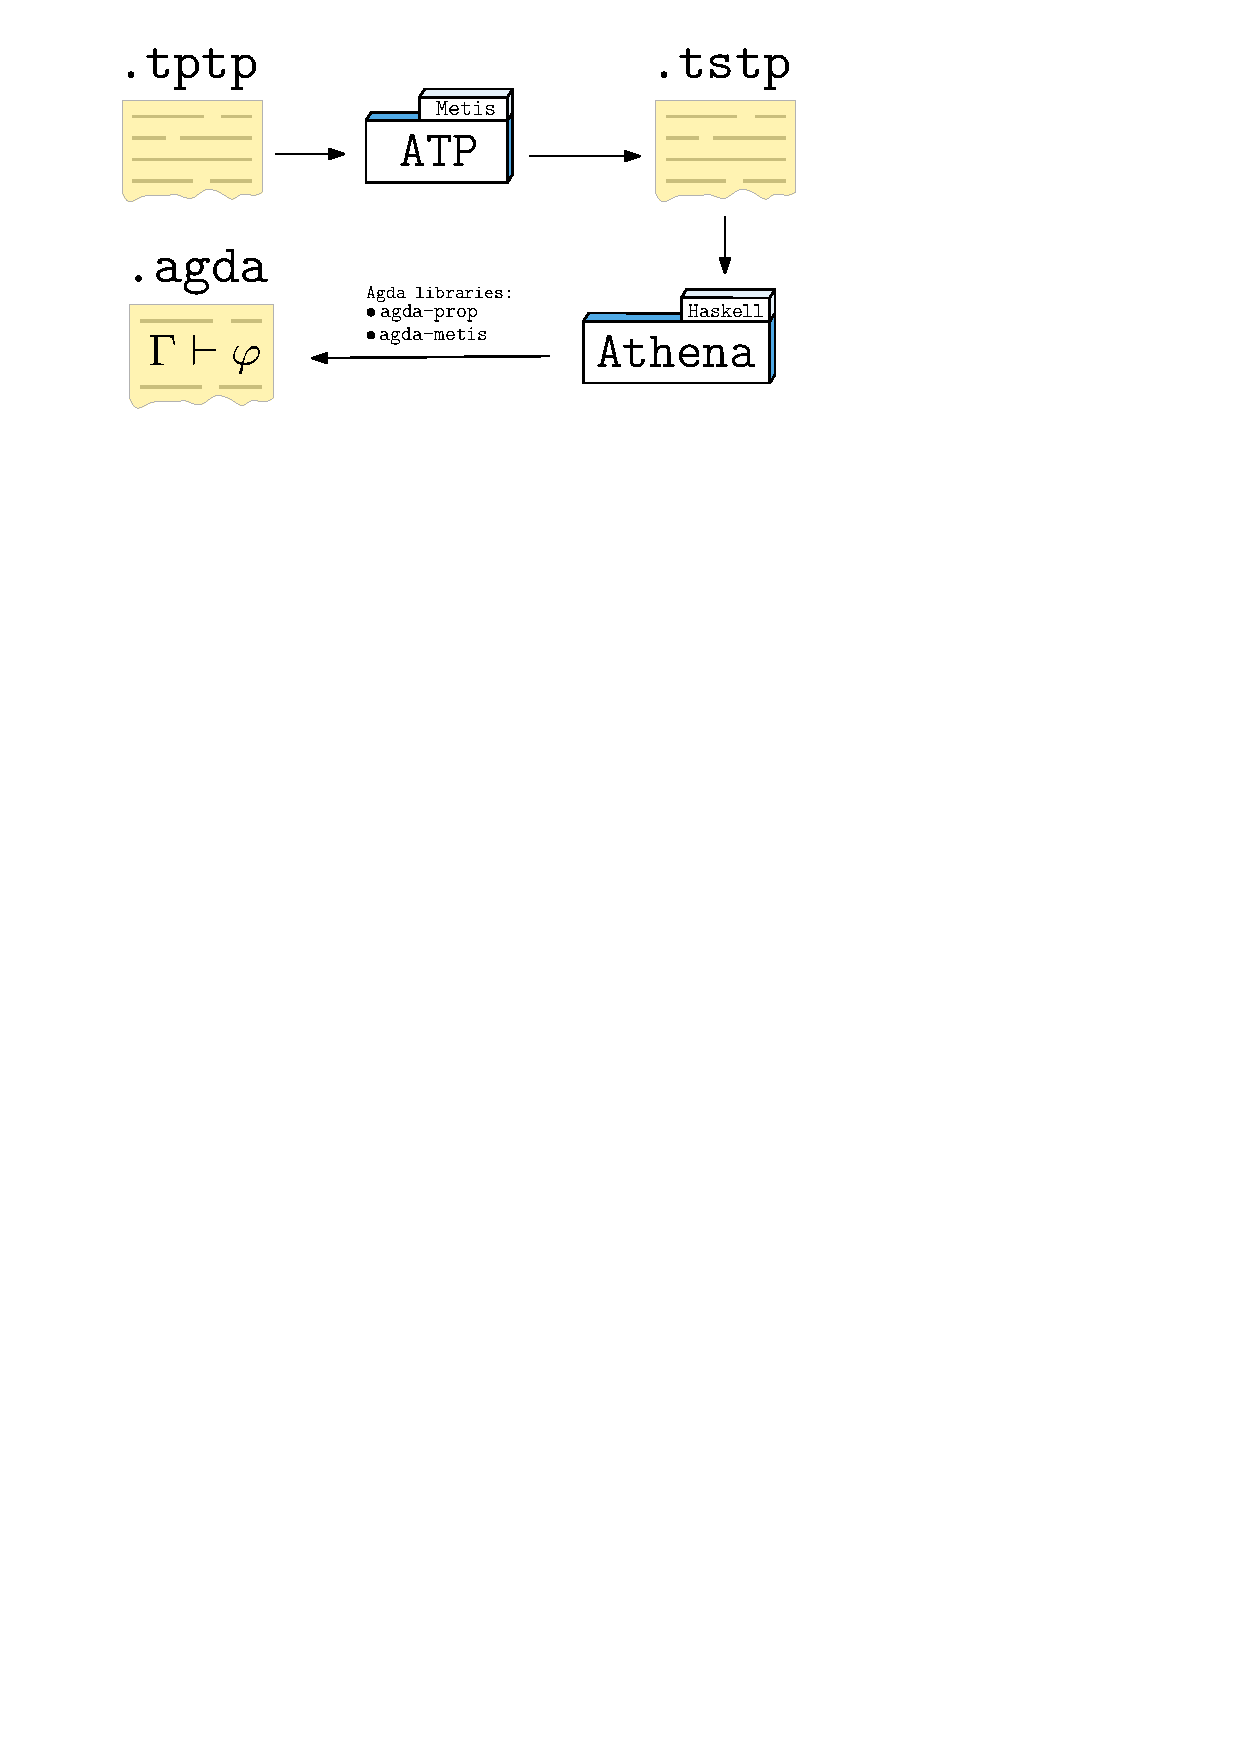
\includegraphics[scale=0.85]{diagram.pdf}
    \label{im:athena}
    \caption{Proof reconstruction work flow.}
  \end{figure}
\end{frame}

\begin{frame}{TPTP}
  Is a text format to encode problems in different theories. Its goal is provide
  a standard for all ATPs in the input file format. The version for derivations
  is named TSTP but this one is not a standard yet.\\[2mm]

  A TPTP file looks like:

  \problemtptp[basic-4.tptp]{../test/prop-pack/problems/basic/basic-4.tptp}{2}

\end{frame}

\begin{frame}{TSTP}
  A derivation of the previous problem output by Metis ATP.
{\footnotesize
  \problemtptp[basic-4.tstp]{../test/prop-pack/problems/basic/basic-4.tstp}{0}
}
\end{frame}

\begin{frame}{Agda}
   A verified proof of the previous derivation output by Athena.

  \begin{figure}
    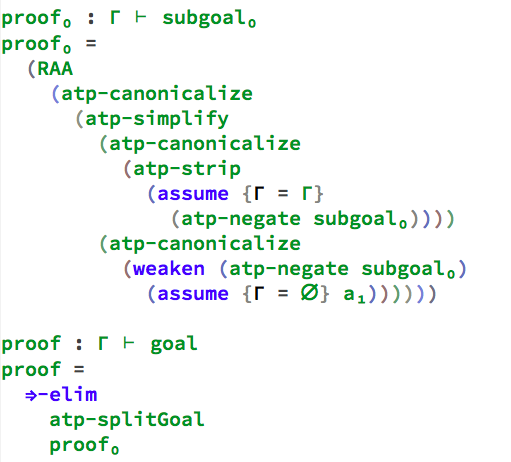
\includegraphics[scale=0.35]{basic-4}
    \label{im:basic}
    \caption{Type-checked Proof.}
  \end{figure}

\end{frame}


\begin{frame}{Natural deduction tree}
  $\Gamma , p \vdash p$
\begin{proof}\hfill
\label{basic-der}
\begin{prooftree}
\AxiomC{$\Gamma \vdash a_1$}
\RightLabel{\scriptsize({\bfseries weaken $\neg\ \text{subgoal}_0$})}
\UnaryInfC{$\Gamma, \neg\ \text{subgoal}_0\,\vdash a_1$}
\RightLabel{\scriptsize({\bfseries canonicalize})}
\UnaryInfC{$\Gamma, \neg\ \text{subgoal}_0\,\vdash p$}
\AxiomC{$\Gamma \vdash p$}
\RightLabel{\scriptsize({\bfseries assume})}
\UnaryInfC{$\Gamma, \neg\ \text{subgoal}_0\,\vdash \neg p$}
\RightLabel{\scriptsize({\bfseries canonicalize})}
\UnaryInfC{$\Gamma, \neg\ \text{subgoal}_0\,\vdash \neg p$}
\RightLabel{\scriptsize({\bfseries simplify})}
\UnaryInfC{$\Gamma, \neg\ \text{subgoal}_0\,\vdash \neg p$}
\BinaryInfC{$\bot$}
\RightLabel{\scriptsize({\bfseries RAA})}
\UnaryInfC{$\Gamma \vdash p$}
\end{prooftree}
% A tree deduction of problem \ref{prob1}
\end{proof}
\end{frame}
% The tool : Athena.
% Its components:
% - agda-prop (logic framework)
% - agda-metis (ATP rules)
% - prop-pack (problems)

\begin{frame}{Future work}

  \begin{itemize}
  \item
    Extend the libraries Agda-Prop and Agda-Metis to handle predicated logic
  \item
    Reconstruct proofs of eprover in Agda-EProver
  \item
    Support more versions of GHC in Athena
  \end{itemize}

\end{frame}


\begin{frame}{References}

\end{frame}

\end{document}
